\documentclass[aspectratio=169]{beamer}
\usepackage[utf8]{inputenc}
\usepackage{booktabs}
\usepackage{graphicx}
\usepackage{amsmath}
\usepackage{tikz}

\usetheme{default}
\definecolor{iitblue}{RGB}{15,58,92}
\setbeamercolor{structure}{fg=iitblue}
\setbeamercolor{frametitle}{bg=iitblue,fg=white}
\setbeamercolor{title}{fg=iitblue}
\setbeamerfont{frametitle}{series=\bfseries}
\setbeamertemplate{navigation symbols}{}
\setbeamertemplate{footline}{%
  \leavevmode
  \hbox{\begin{beamercolorbox}[wd=1\paperwidth,ht=2.7ex,dp=1ex,leftskip=1em,rightskip=1em]{iitblue}
  \usebeamercolor[fg]{structure}\color{white}\scriptsize
  Department of Physics, Indian Institute of Technology, Bhubaneswar
  \hfill \insertframenumber
  \end{beamercolorbox}}%
}
\setbeamertemplate{itemize item}{\color{iitblue}\textbullet}
\setbeamertemplate{itemize subitem}{\color{iitblue}\textendash}

\title{\textbf{Design of a Hamiltonian-Based Vision Kernel (HVK)\\[2pt]\large using a Hybrid Architecture and Tensor Network Framework}}
\author{Sparsho Chakraborty}
\institute{Department of Physics, Indian Institute of Technology, Bhubaneswar}
\date{July 14, 2026}

\begin{document}

% ---------- 1: Title ----------
\begin{frame}
\titlepage
\end{frame}

% ---------- 2: Overview ----------
\begin{frame}{Overview}
\begin{enumerate}
  \item Motivation \& Idea
  \item Pipeline \& Image Preparation
  \item Results: Reconstruction Demos
  \item Sanity Checks \& Diagnostics
  \item Quantitative Results
  \item Does the Quantum Part Actually Help?
  \item Conclusion
\end{enumerate}
\end{frame}

% ---------- 3: Motivation & Idea ----------
\begin{frame}{Motivation \& Idea}
\begin{itemize}
  \item Quantum models for high-definition images: too many qubits, too much circuit depth.
  \item High-dimensional data needs compression \emph{without} losing correlation and fidelity.
  \item \textbf{Our approach:} patch decomposition $\to$ MPS compression $\to$ quantum feature extraction $\to$ classical decoder.
  \item A learnable Heisenberg energy term adds a physics-inspired inductive bias.
\end{itemize}
\end{frame}

% ---------- 4: Model Pipeline (KEPT UNCHANGED) ----------
\begin{frame}[plain]
\begin{tikzpicture}[remember picture, overlay]
\node[at=(current page.center)] {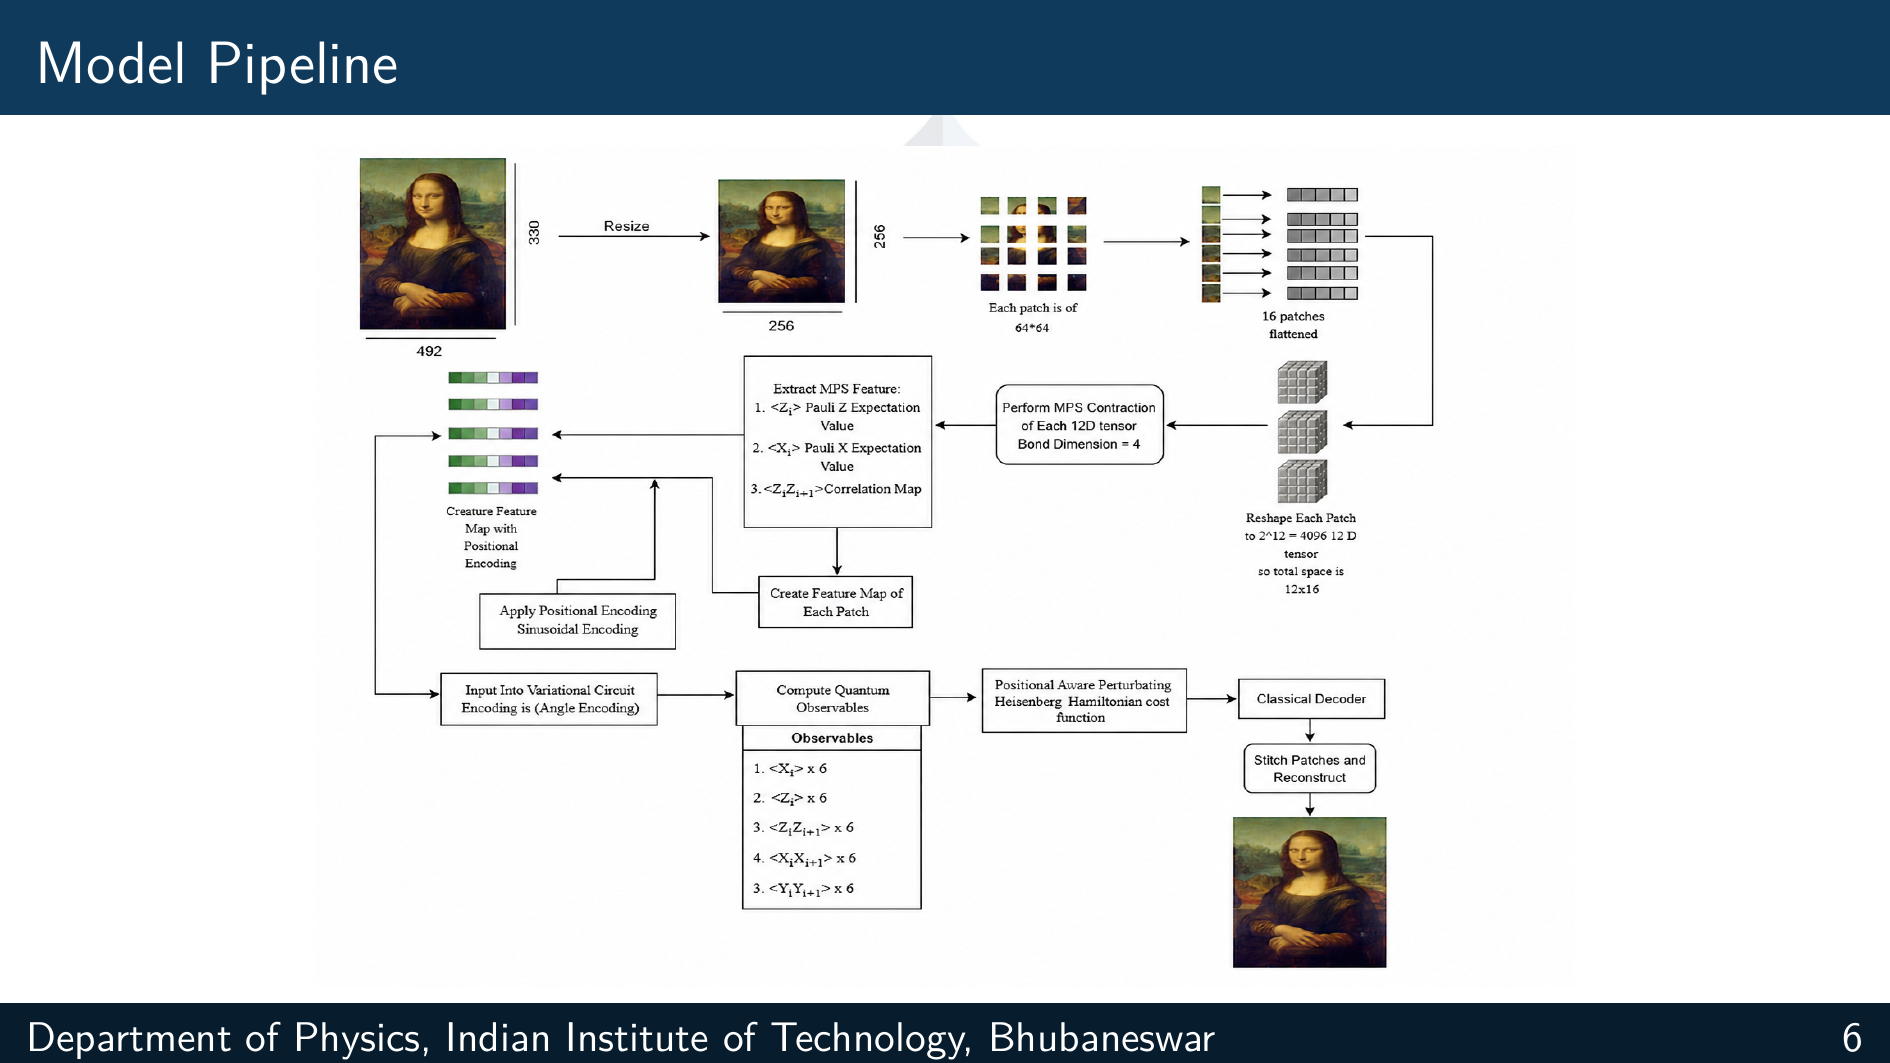
\includegraphics[width=\paperwidth,height=\paperheight]{figures/kept_model_pipeline-06.png}};
\end{tikzpicture}
\end{frame}

% ---------- 5: Positional Encoding / Image Preparation (KEPT UNCHANGED) ----------
\begin{frame}[plain]
\begin{tikzpicture}[remember picture, overlay]
\node[at=(current page.center)] {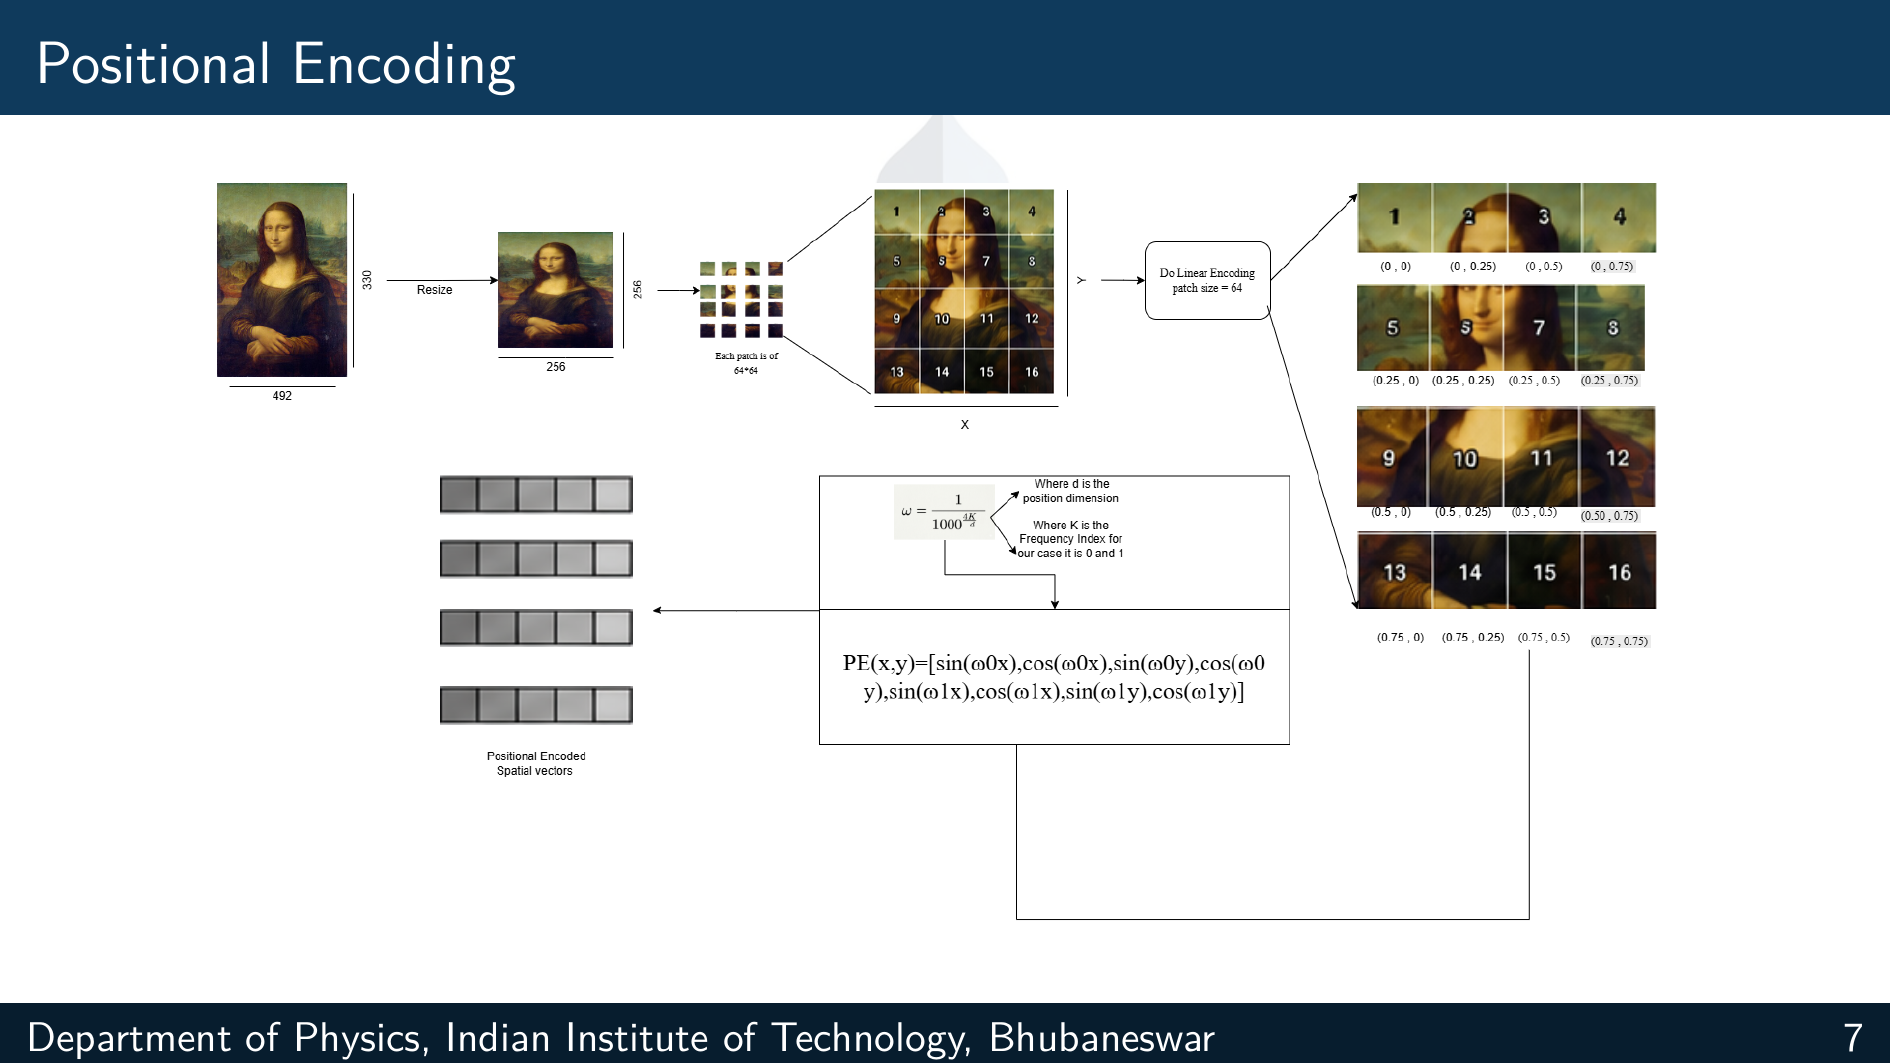
\includegraphics[width=\paperwidth,height=\paperheight]{figures/kept_positional_encoding-07.png}};
\end{tikzpicture}
\end{frame}

% ---------- 6: Reconstruction without Hamiltonian kernel ----------
\begin{frame}[plain]
\begin{tikzpicture}[remember picture, overlay]
\node[at=(current page.center)] {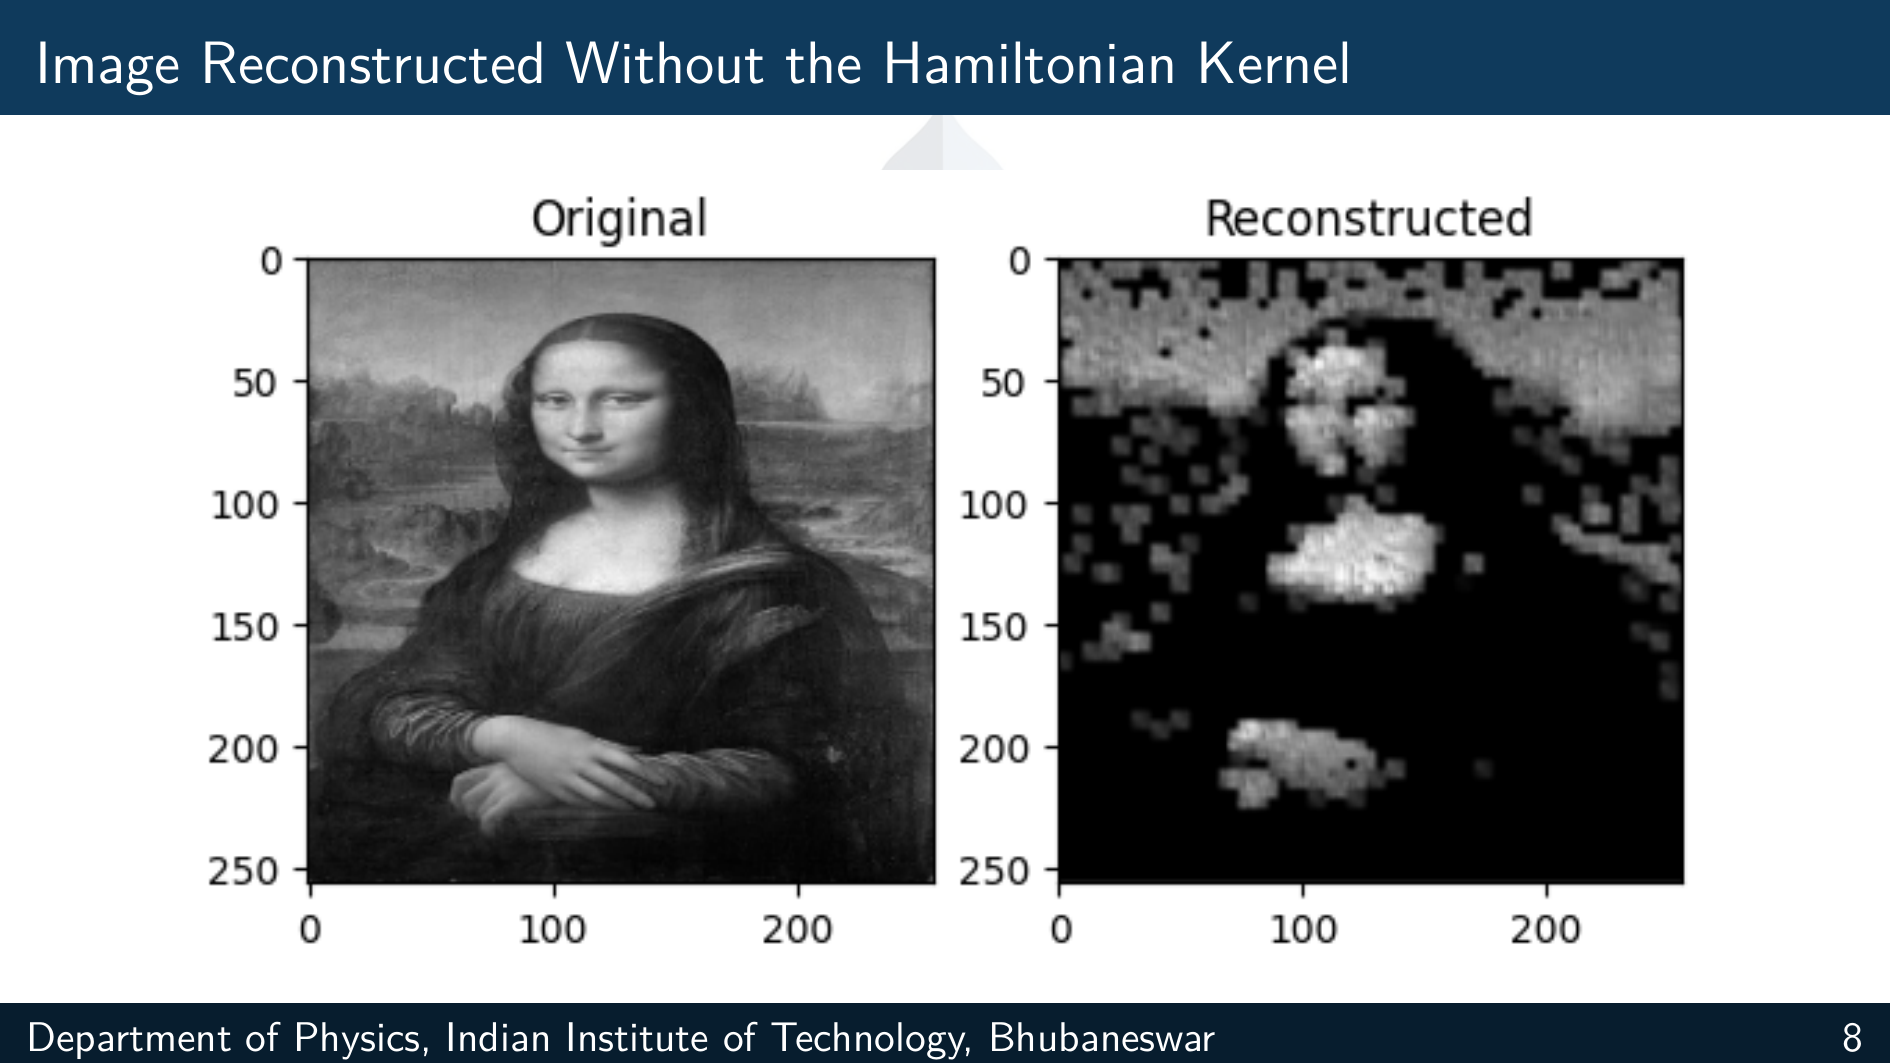
\includegraphics[width=\paperwidth,height=\paperheight]{figures/kept_page-08.png}};
\end{tikzpicture}
\end{frame}

% ---------- 7: Reconstruction with positional field only ----------
\begin{frame}[plain]
\begin{tikzpicture}[remember picture, overlay]
\node[at=(current page.center)] {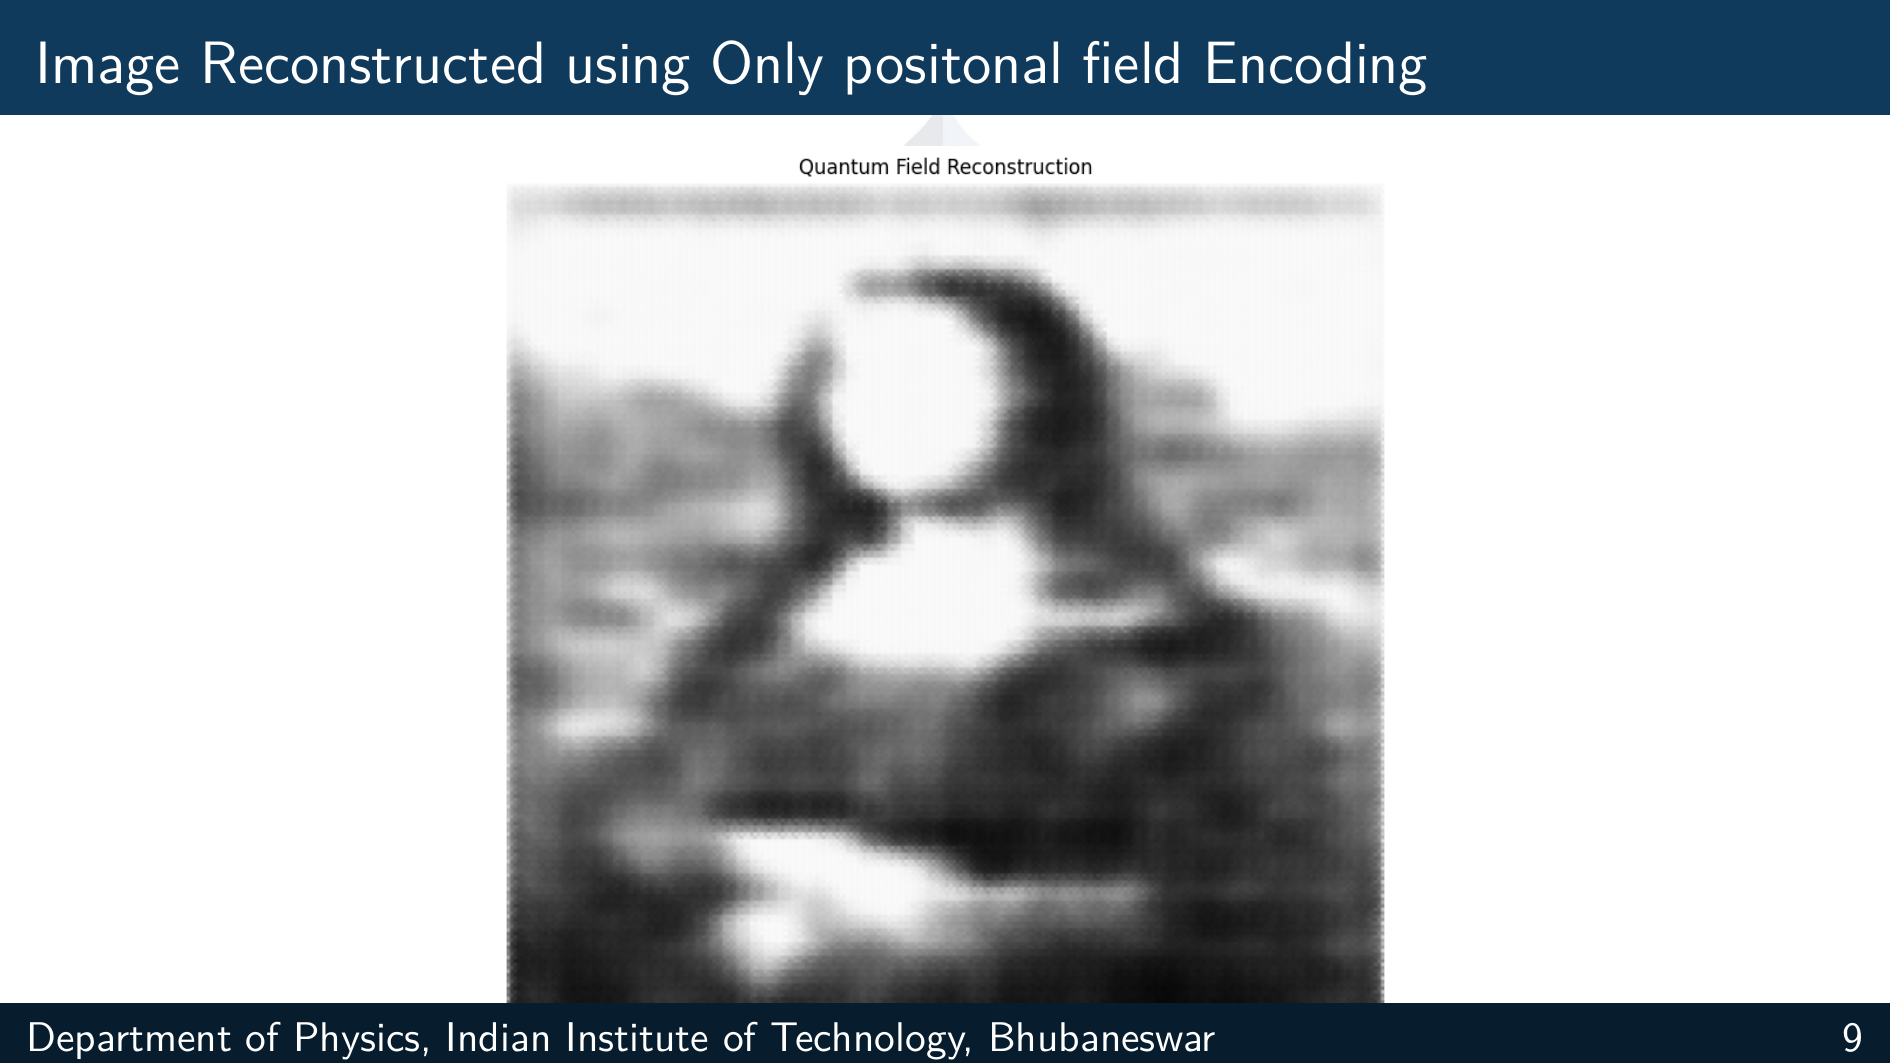
\includegraphics[width=\paperwidth,height=\paperheight]{figures/kept_page-09.png}};
\end{tikzpicture}
\end{frame}

% ---------- 8: Full HVK reconstruction (payoff) ----------
\begin{frame}[plain]
\begin{tikzpicture}[remember picture, overlay]
\node[at=(current page.center)] {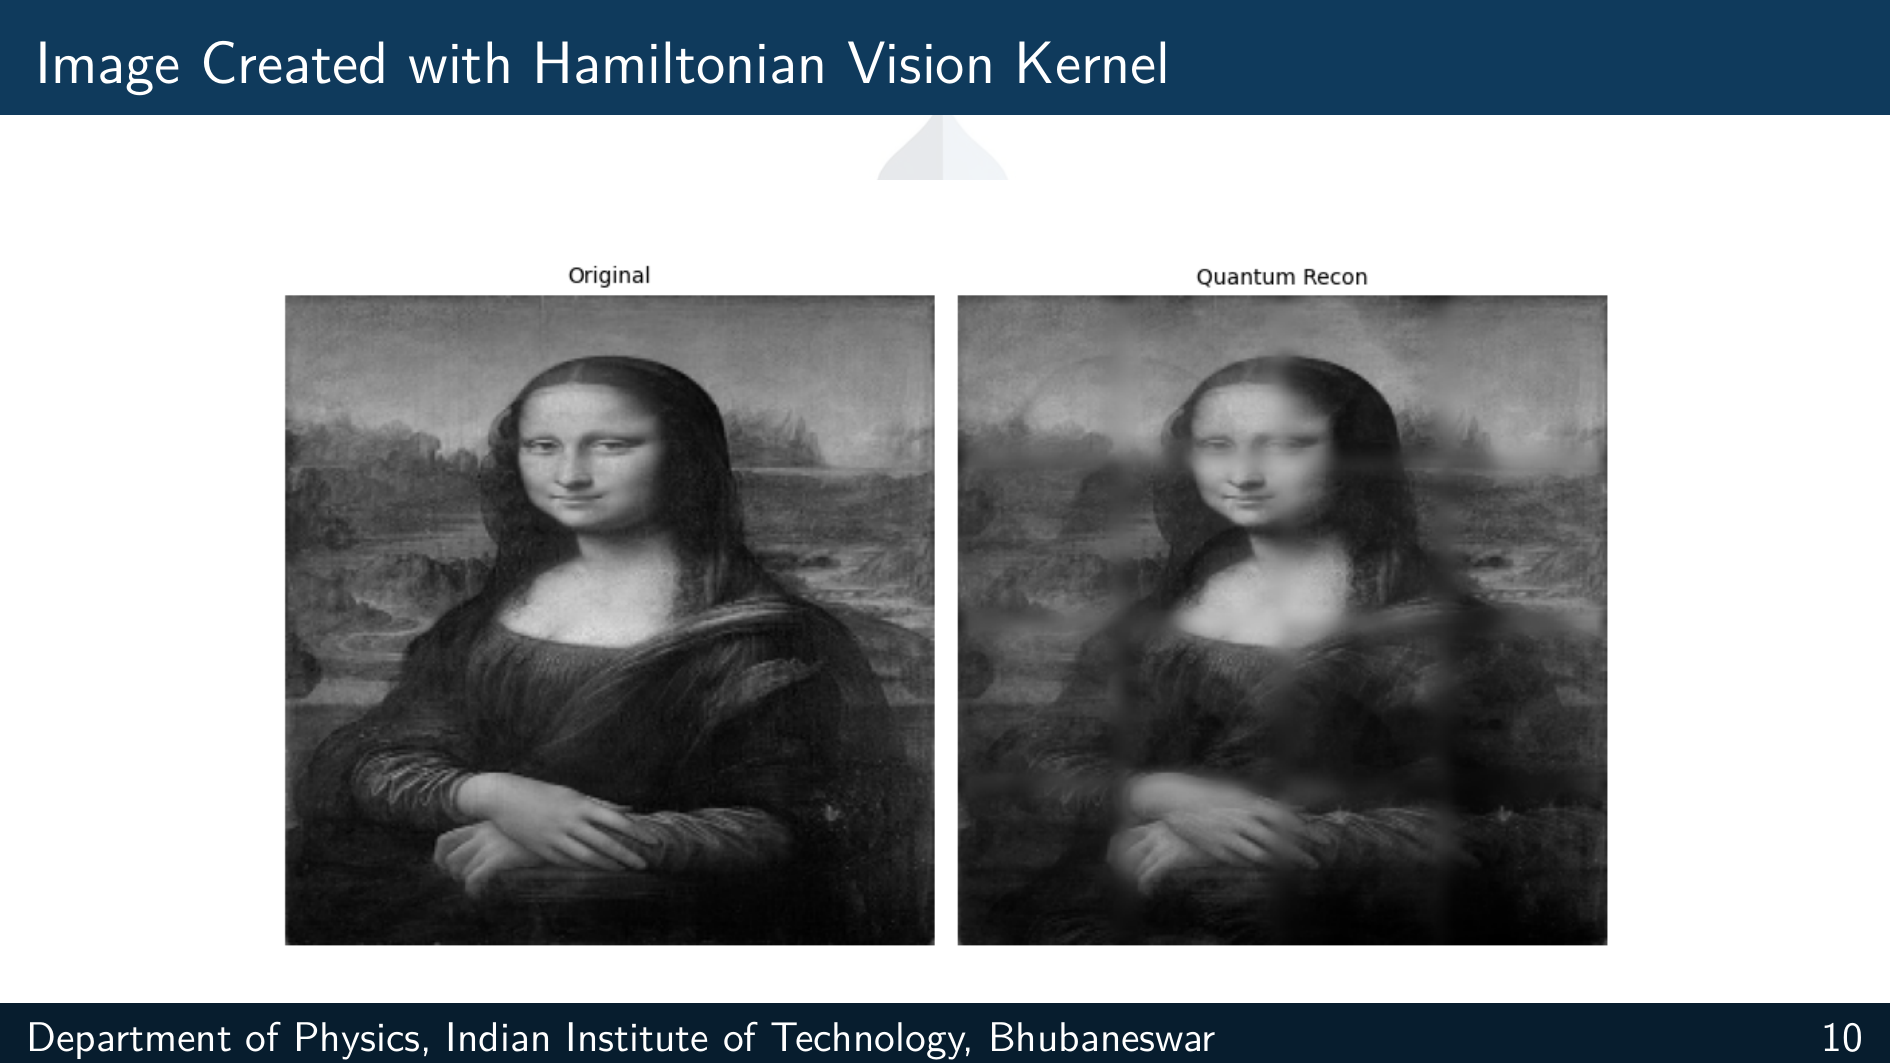
\includegraphics[width=\paperwidth,height=\paperheight]{figures/kept_page-10.png}};
\end{tikzpicture}
\end{frame}

% ---------- 9: Random / zero latent sanity check ----------
\begin{frame}[plain]
\begin{tikzpicture}[remember picture, overlay]
\node[at=(current page.center)] {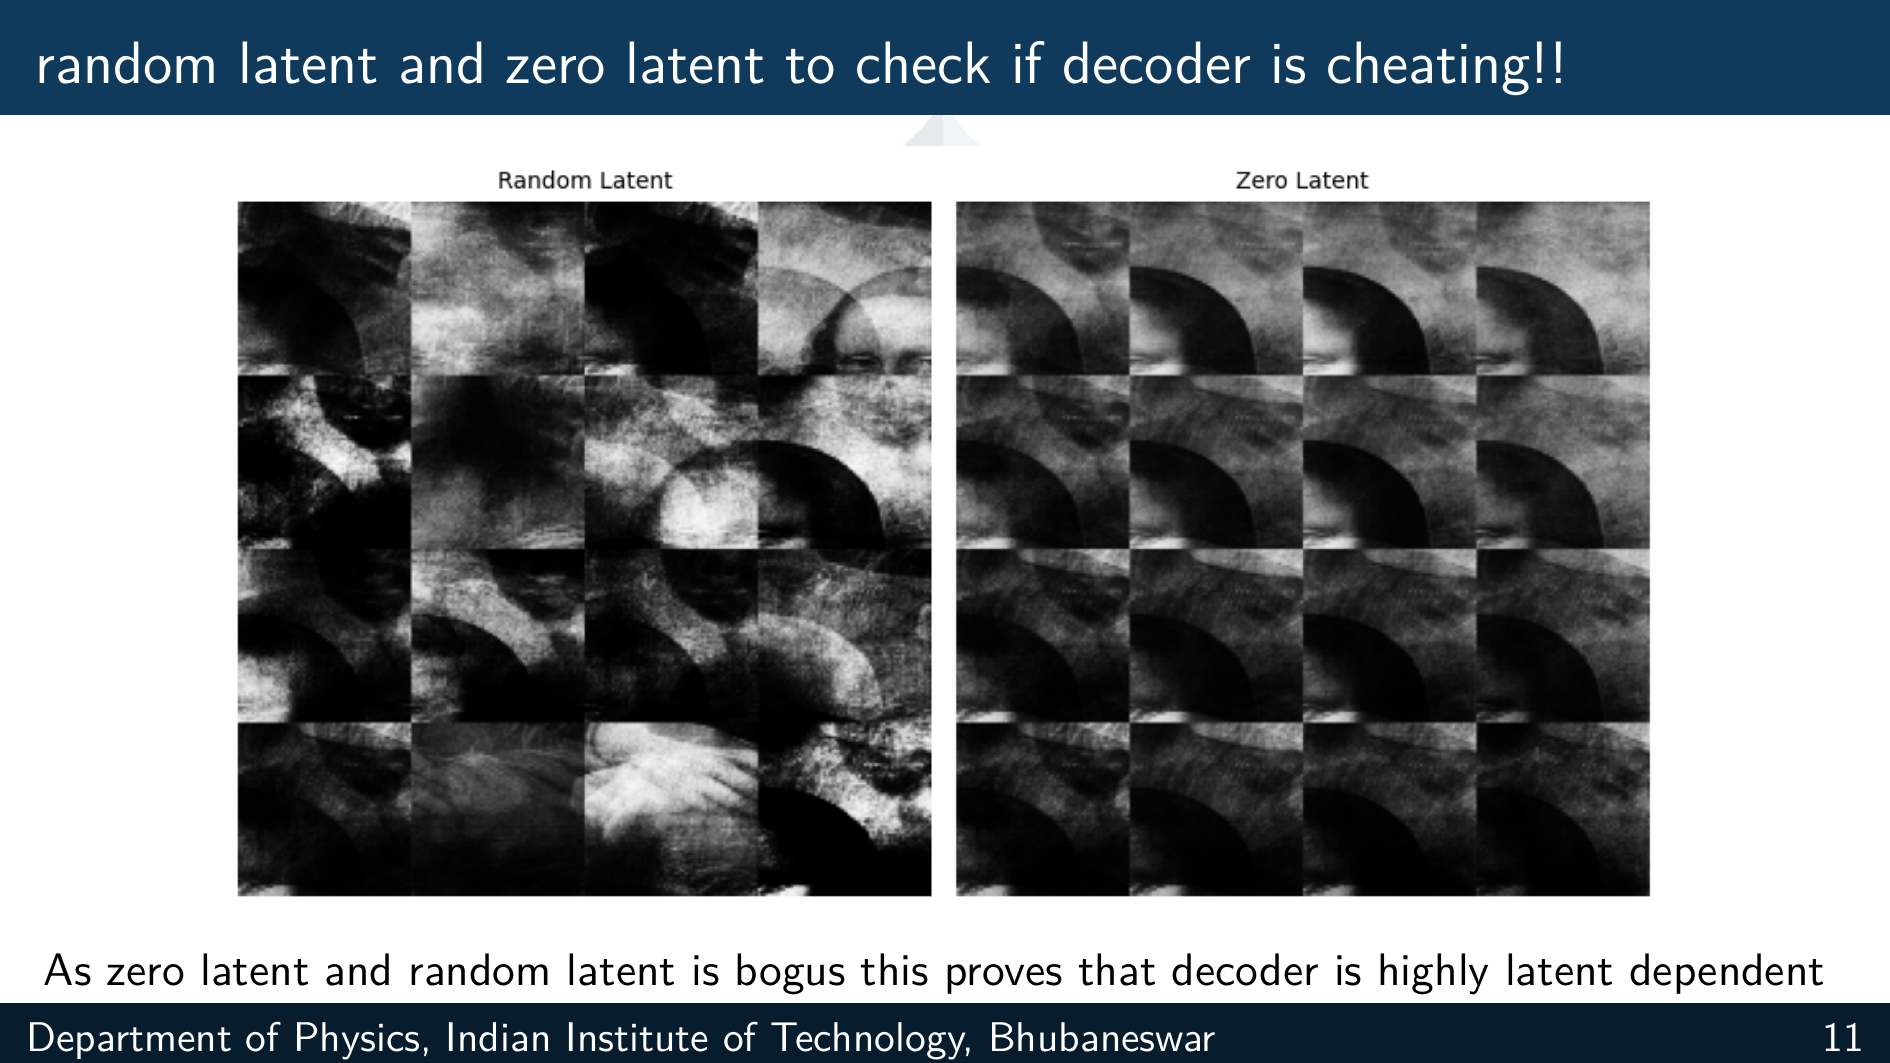
\includegraphics[width=\paperwidth,height=\paperheight]{figures/kept_page-11.png}};
\end{tikzpicture}
\end{frame}

% ---------- 10: Observable distribution ----------
\begin{frame}[plain]
\begin{tikzpicture}[remember picture, overlay]
\node[at=(current page.center)] {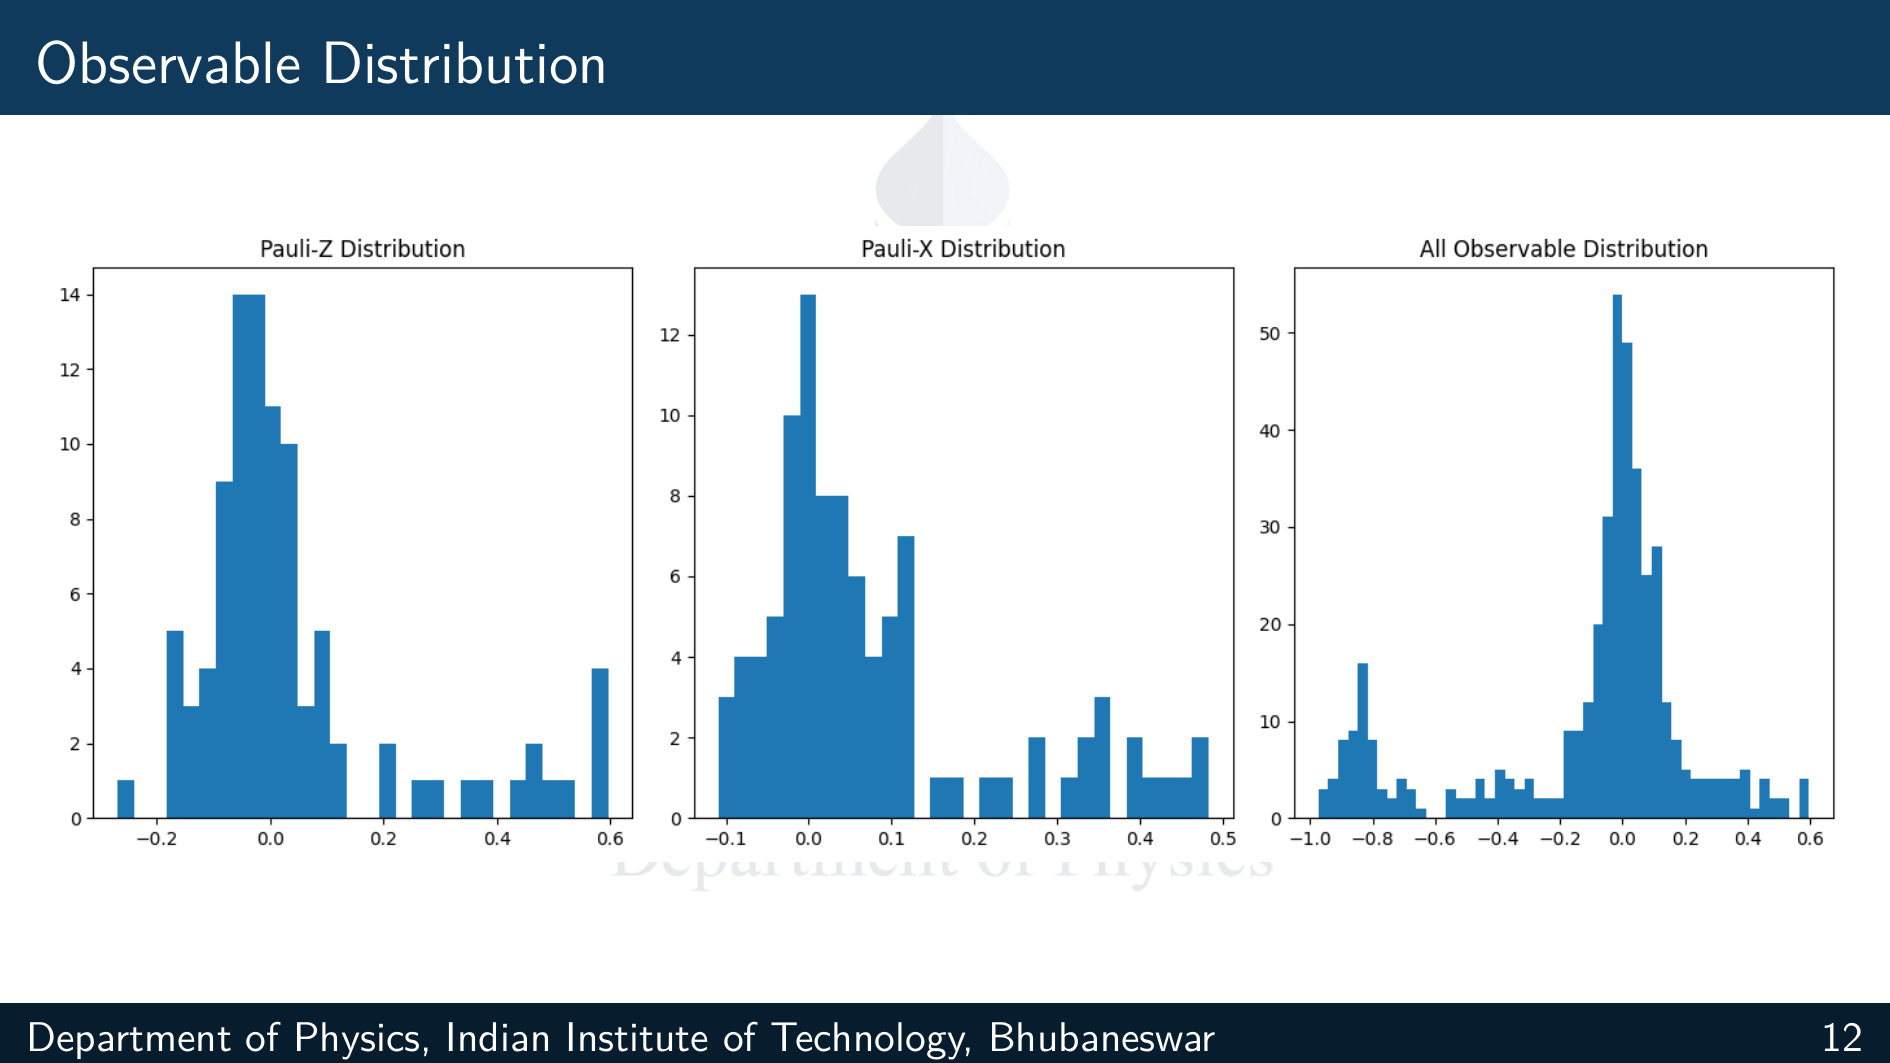
\includegraphics[width=\paperwidth,height=\paperheight]{figures/kept_page-12.png}};
\end{tikzpicture}
\end{frame}

% ---------- 11: Correlation matrix ----------
\begin{frame}[plain]
\begin{tikzpicture}[remember picture, overlay]
\node[at=(current page.center)] {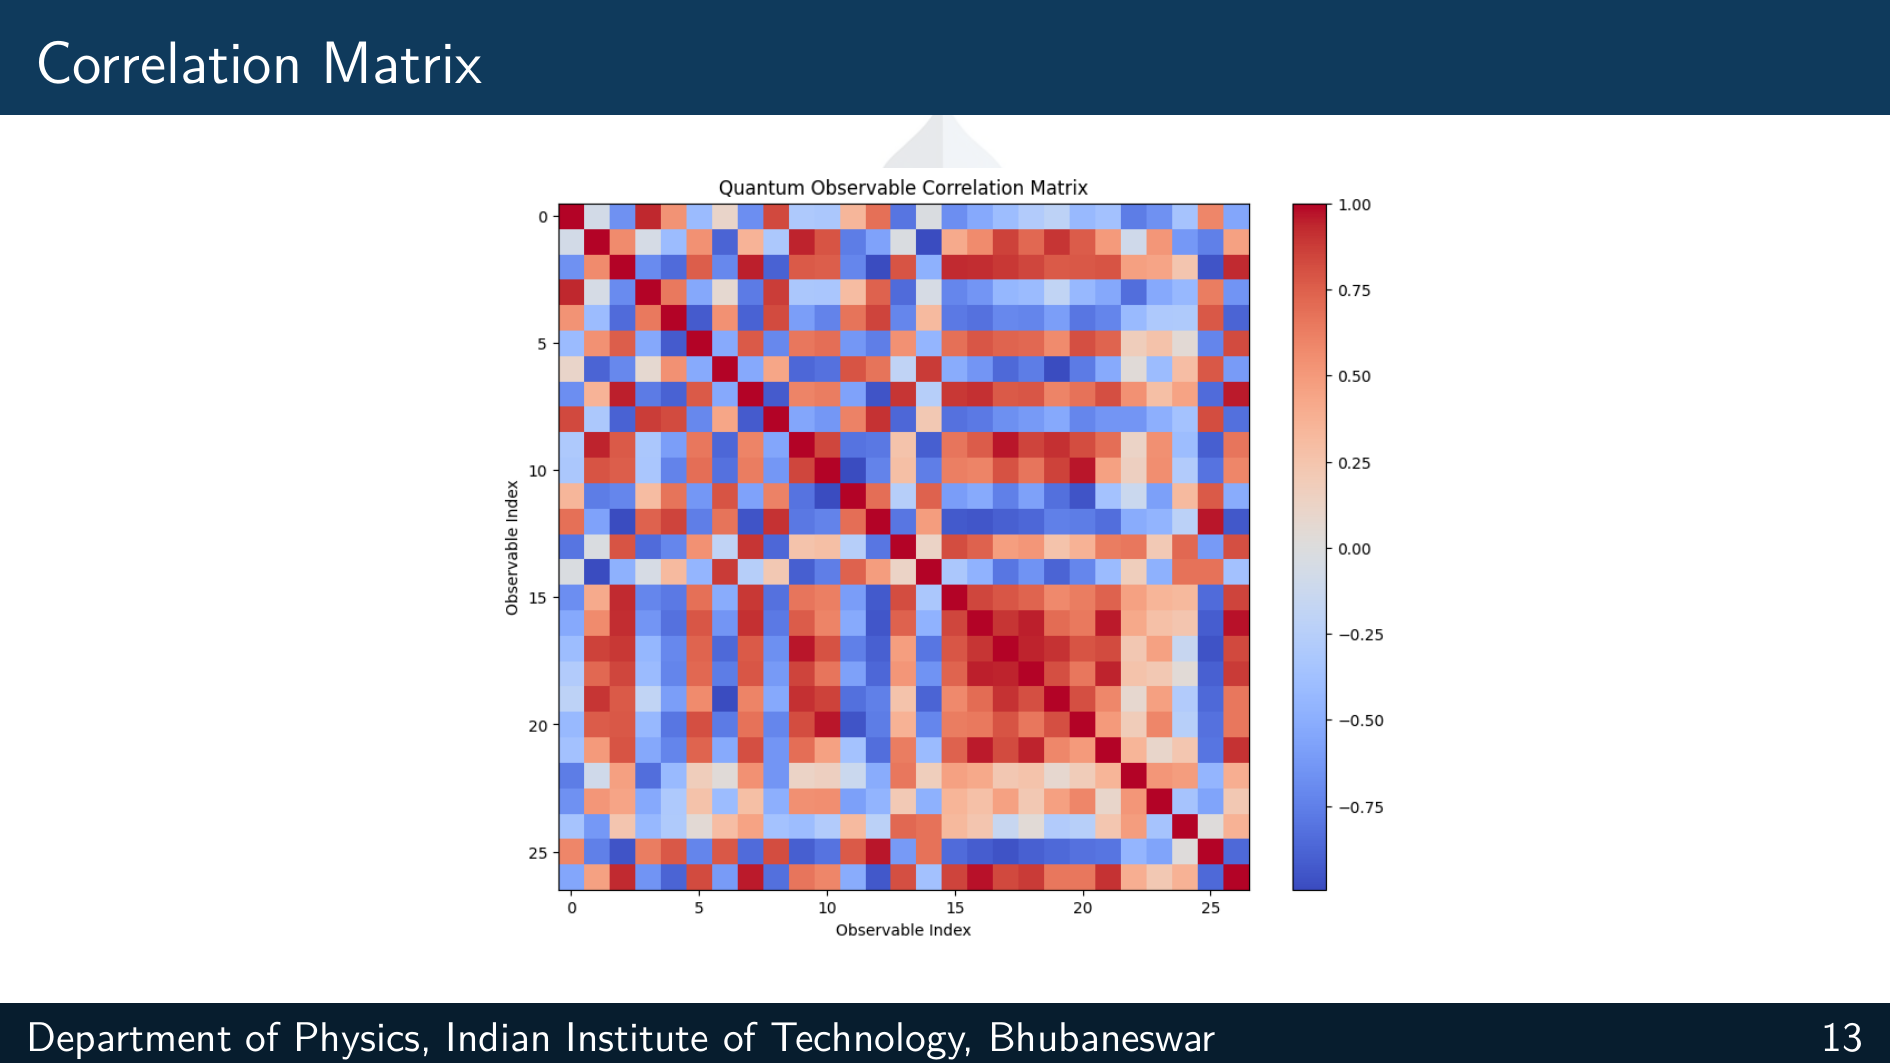
\includegraphics[width=\paperwidth,height=\paperheight]{figures/kept_page-13.png}};
\end{tikzpicture}
\end{frame}

% ---------- 12: Positional encoding heat map ----------
\begin{frame}[plain]
\begin{tikzpicture}[remember picture, overlay]
\node[at=(current page.center)] {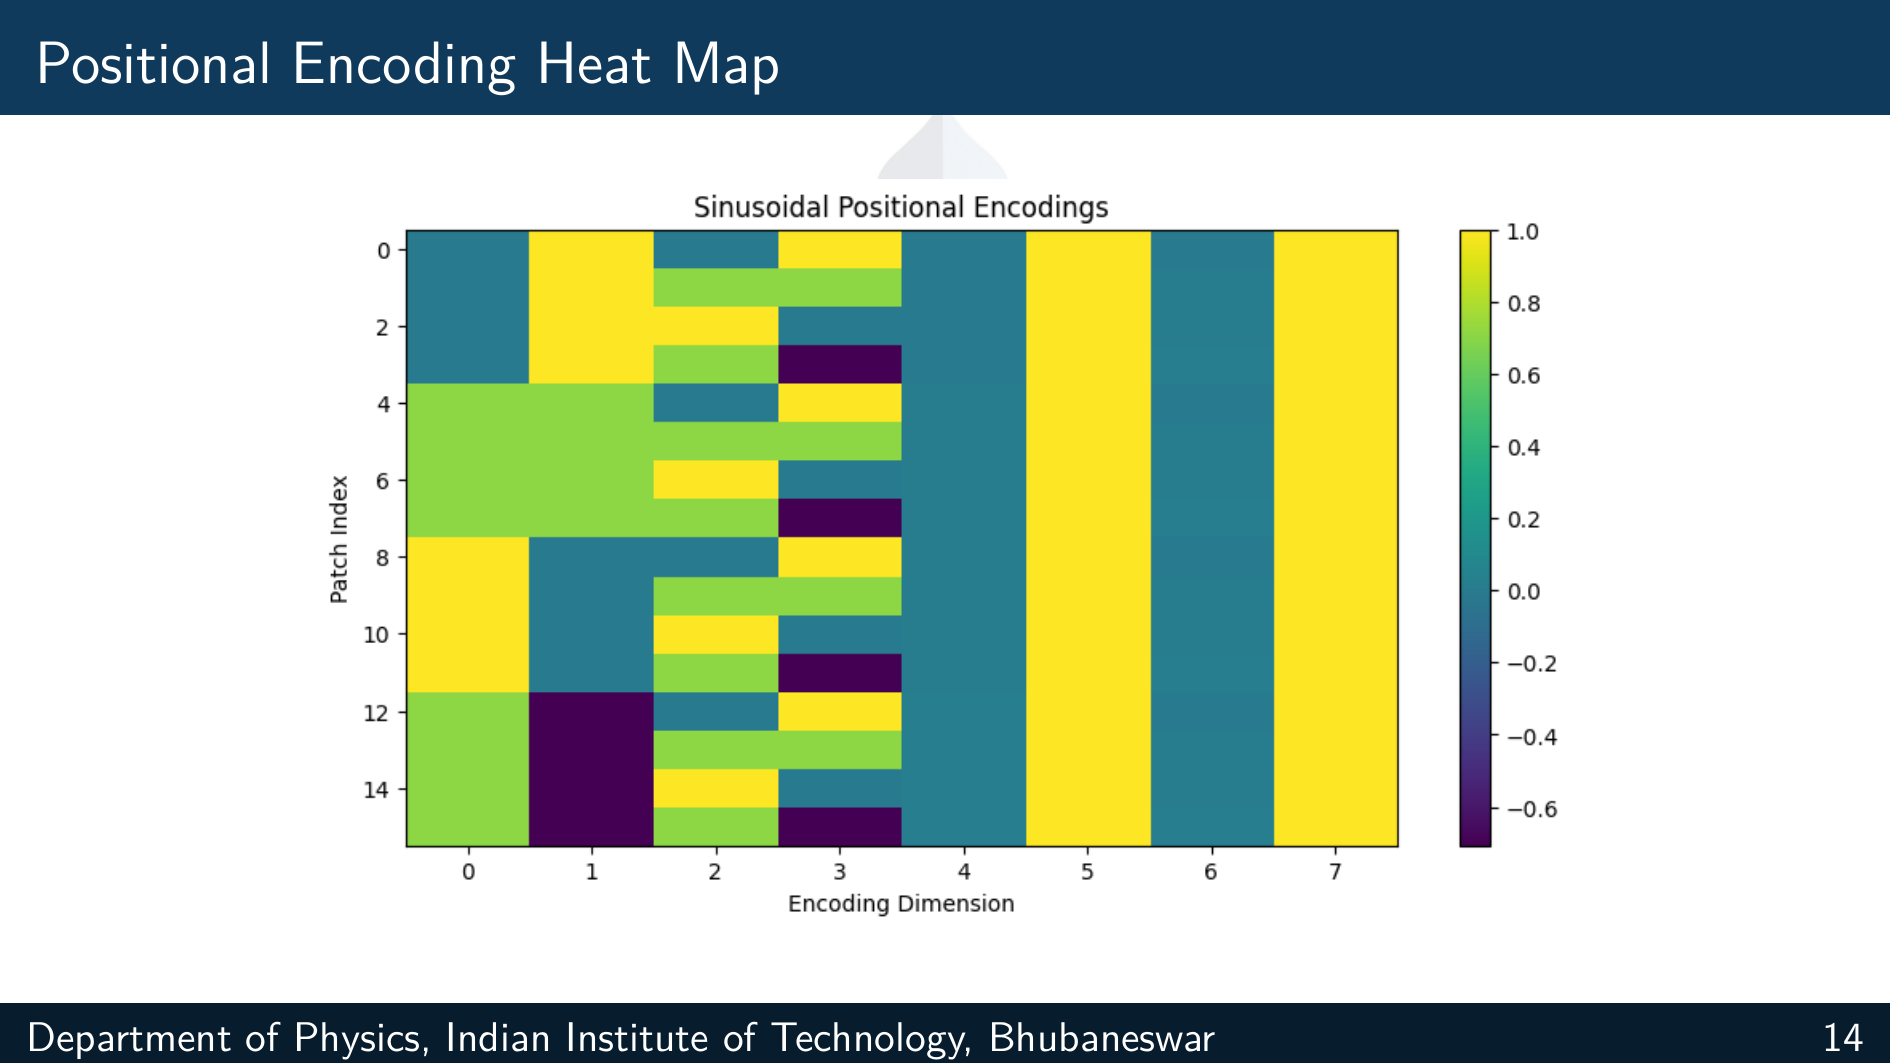
\includegraphics[width=\paperwidth,height=\paperheight]{figures/kept_page-14.png}};
\end{tikzpicture}
\end{frame}

% ---------- 13: Quantitative results ----------
\begin{frame}{Quantitative Results (Monalisa Demo)}
\centering\scriptsize
\begin{tabular}{lc}
\toprule
Metric & Value \\
\midrule
MSE & $1.953763\times10^{-3}$ \\
MAE & $3.166284\times10^{-2}$ \\
PSNR & $27.09128$ dB \\
Total Parameters & $1.090691\times10^{6}$ \\
Model Parameters & $387$ \\
Decoder Parameters & $1.090304\times10^{6}$ \\
Observable Mean & $-1.053798\times10^{-1}$ \\
Observable Std & $3.428020\times10^{-1}$ \\
Mean Entropy & $9.944191\times10^{-3}$ \\
Max Entropy & $1.364326\times10^{-1}$ \\
Mean Energy & $-2.525678$ \\
Std Energy & $1.780927\times10^{-1}$ \\
\bottomrule
\end{tabular}
\end{frame}

% ---------- 14: Segue into the ablation study ----------
\begin{frame}{Does the Quantum Part Actually Help?}
\begin{itemize}
  \item The demo above shows HVK \emph{reconstructs} images well.
  \item It does not show \emph{which component} is responsible.
  \item So we ran a resource-matched, freeze-based, multi-seed ablation study.
\end{itemize}
\vfill
\centering\textbf{This is what we found.}
\end{frame}

% ---------- 15: Key ablation finding ----------
\begin{frame}{What We Found: The Classical Decoder Does the Work}
\centering\scriptsize
\begin{tabular}{lcc}
\toprule
Variant (Monalisa, 5 seeds) & PSNR (dB) & Verdict \\
\midrule
Freeze classical, train quantum & $10.93\pm0.00$ & Collapses \\
Shared VQC baseline & $32.97\pm0.22$ & Reference \\
No entanglement / No MPS & $\approx 33.0$ & Not significant \\
Classical tanh replacement & $33.50\pm0.00$ & Exceeds baseline \\
\bottomrule
\end{tabular}

\vspace{6pt}
Held-out CIFAR-10: raw-linear ($18.80\pm1.42$ dB) beats trained HVK2D ($18.12\pm1.54$ dB), $p=9.5\times10^{-6}$.

\vspace{6pt}
\begin{itemize}\scriptsize
  \item We also caught and withdrew a leakage bug in an early diagnostic (a too-good-to-be-true $R^2=1.0$).
  \item Two narrow positive results survive: entanglement is necessary on a synthetic pair-correlation task, and a $D_4$-pooled variant is provably symmetric.
\end{itemize}
\end{frame}

% ---------- 16: Conclusion ----------
\begin{frame}{Conclusion}
\begin{itemize}
  \item HVK reconstructs images well and its representation is physically interpretable.
  \item But on held-out real images, the classical decoder --- not the quantum circuit --- is load-bearing.
  \item We report this honestly, because the evaluation protocol is the real contribution.
\end{itemize}
\end{frame}

% ---------- 17: Thank you ----------
\begin{frame}[plain]
\begin{center}
\vspace{2cm}
{\Huge \textbf{THANK YOU!}}
\vspace{1cm}


\includegraphics[width=2cm]{figures/iitbbslogo.png}
\end{center}
\end{frame}

\end{document}
